% Copyright (C) 2007 Thomas L. Kula
% All Rights Reserved
%
% See the file LICENSE for license terms.
\documentclass[12pt]{article}
\usepackage{graphicx}
\setlength{\paperwidth}{5.5in}
\setlength{\paperheight}{8.5in}
\setlength{\textheight}{6.45in}
\setlength{\oddsidemargin}{-0.5in}
\setlength{\evensidemargin}{-0.5in}
\setlength{\textwidth}{4.0in}
\setlength{\parindent}{0in}
\setlength{\parskip}{3mm}
\usepackage[print]{booklet} \nofiles
\source{\magstep0}{5.5in}{8.5in}
\target{\magstep0}{11in}{8.5in}
\setpdftargetpages
\begin{document}

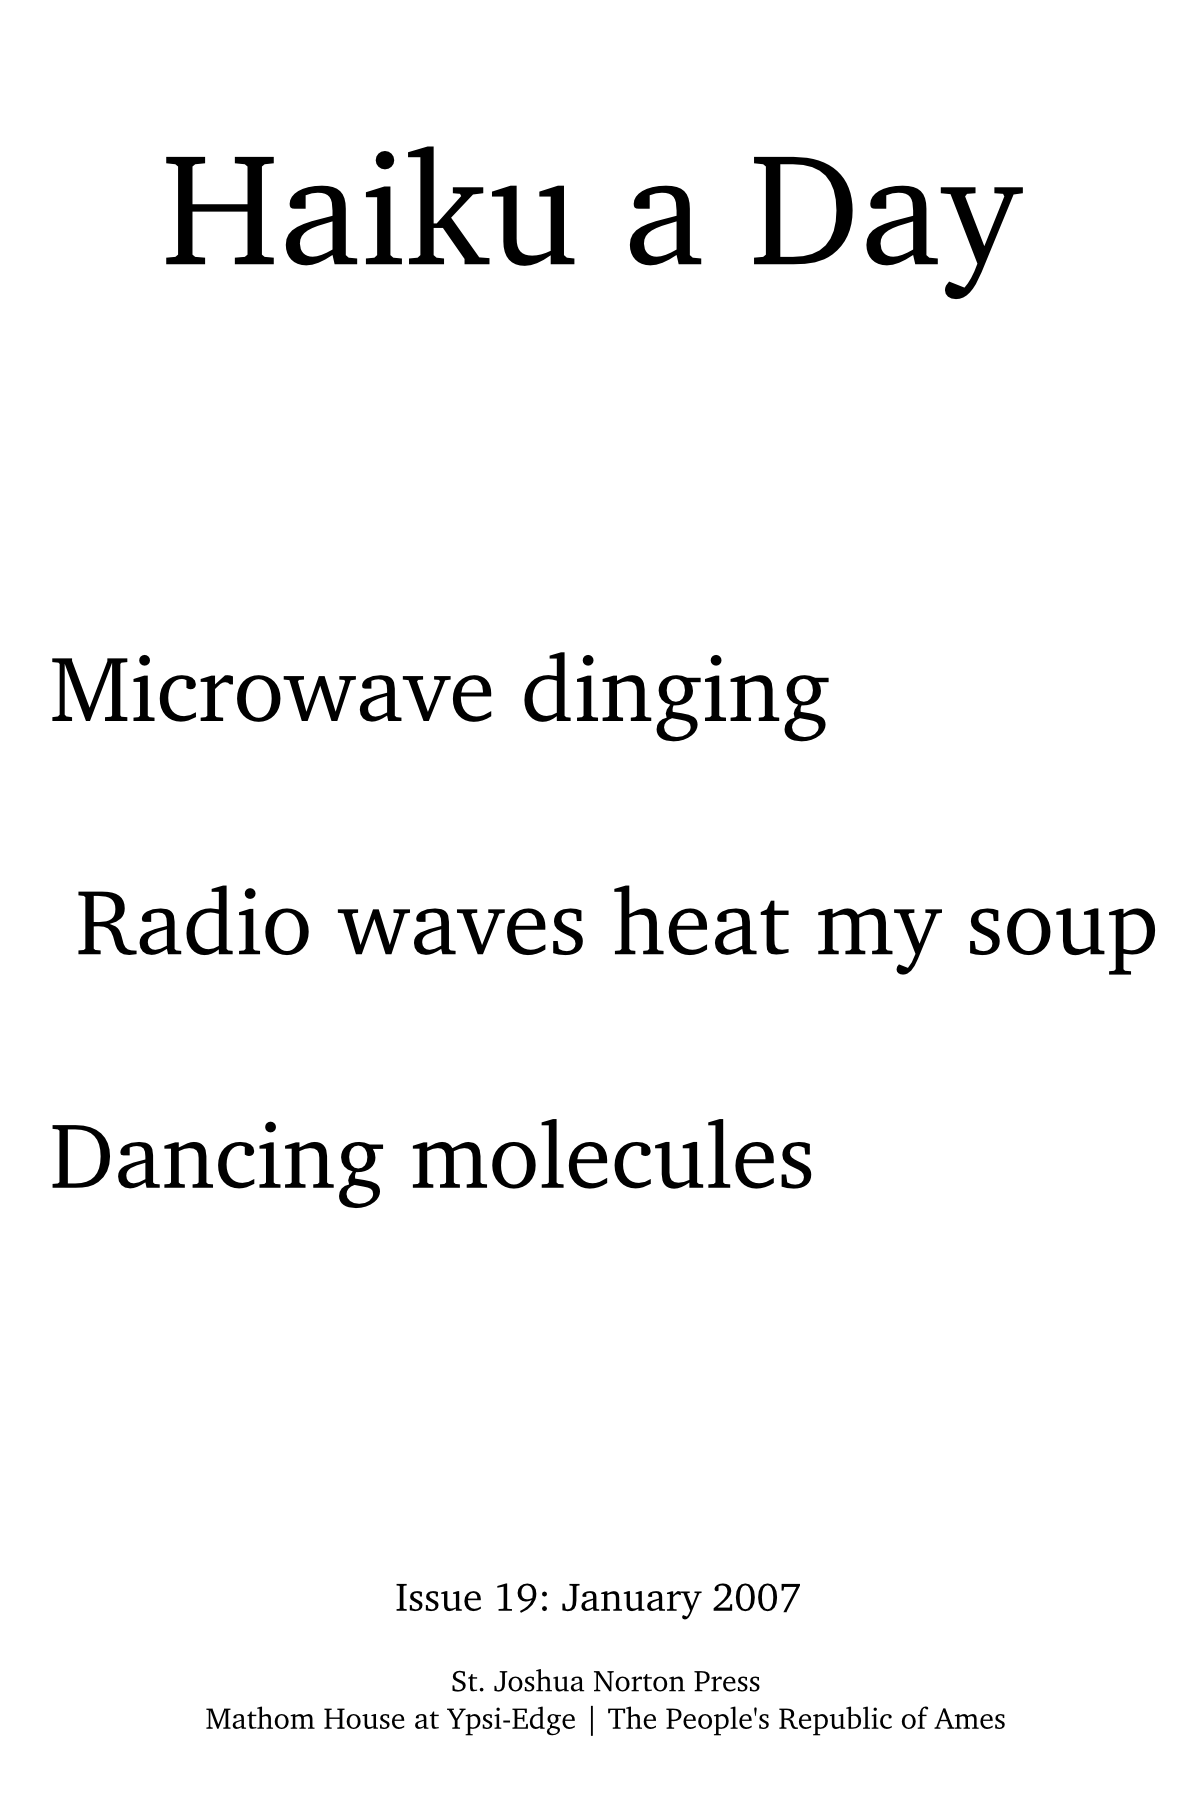
\includegraphics[width=101mm]{frontpage.png}

\newpage

I'm putting the zine together, and at the same time enjoying
a bowl of soup (as you may have gathered from the cover haiku, or,
as we in the biz call it, the coverku) and I'm struck by the
miracle that is Soup.

Seriously, you chop up a bunch of stuff, put it in a big pot,
add liquid, and simmer it for several hours. It's a minor
miracle, that a process so simple can make something so good.
If I were one for starting religious cults, I'd make one 
based on soup.

Who am I kidding? I {\em am} one for starting religious cults.

Note the new address on the back. 

--- Thomas

http://kula.tproa.net/had/ \\
kula@tproa.net

Download this and previous HADs at the website, so you can
print out you own (DIY, yeah!) or if you want me to send
you one, send me your address, and maybe a stamp if you
are feeling nice. Or send me something you've made.

\setlength{\parskip}{1mm}

1 January 2007

Once more 'round the Sun \\
Circles have no start, no end \\
Yet we mark one here


\newpage

2 January 2007

Quiet night steals sleep \\
Throws it away restlessly \\
Laughing all the way

3 January 2007

When I fall asleep \\
Do those last thoughts go to a \\
Graveyard of ideas?

4 January 2007

Puddles form outside \\
A tiny ocean of life \\
Born, lives, fades away 

5 January 2007

Bang clang shudder boom \\
Music my apartment makes \\
When the heat turns on

6 Janaury 2007

Streets to streets to streets \\
Aimless wandering at night \\
Finding my way home

7 January 2007

Molecules excite \\
Atoms drop energy and \\
Photons create light


\newpage

8 January 2007

Flakes of water fall \\
Specks glide from on high gently \\
To caress the Earth

9 January 2007

Short Cinema Slam \\
Movies made by local folk \\
Besting Hollywood 

10 January 2007

Into the sunset \\
Day goes quietly to bed \\
While Night takes it's hold 

11 January 2007

Off to Sirius \\
Dear Robert Anton Wilson. \\
Can you see the Fnords?

12 January 2007

Shoe canvas worn thin \\
A tiny toe tries escape \\
Little pig can't go

13 Janaury 2007

Seeds become flowers \\
Blowing in a cool spring field \\
Dancing to the wind


\newpage

14 January 2007

Cold black ice falling \\
Tiny bits of dust incandesce \\
Streaking through the sky

15 January 2007

Crystaline tree limbs \\
Tinkle as the wind sways them \\
Dropping jewels of ice

16 January 2007

Dark infinite pools \\
A glimmer of light within \\
Pierces deep your soul

17 January 2007

A missing dongle \\
Keeps the intarwebs away \\
Saddening Deejoe

18 January 2007

Scintillating tubes \\
Calling out to travelers \\
``Your turn was back there"

19 January 2007

Gliding on the bridge \\
The bus turns east to the sun \\
And faces the dawn


\newpage

20 January 2007

Behold! The eastern sky \\
Glows with the lights of Detroit \\
Poisoning the stars

21 January 2007

I am Yellow Cake \\
Sweet of Sweets. Look upon my \\
Frosting and dispair 

22 January 2007

Boxes hold many things \\
None of them hold the wires \\
For my phonograph

23 January 2007

The in-head concert \\
Music floating through my brain \\
A song on repeat

24 January 2007

Concrete barrier \\
Tree pushes and bends to you \\
Someday you will yield 

25 January 2007

Carpet fuzz gathers \\
Mount an assault on the hall \\
The vacuum triumps!


\newpage

26 January 2007

Nature's miracle \\
Hard kernels become airy \\
Popcorn, I love you

27 January 2007

Sleepy brain gone dull \\
This latte is not helping \\
Hate meta haiku

28 January 2007

Sad alternator \\
My car's battery goes dull \\
When you don't fill it

29 January 2007

A hail of bullets \\
Nerf pellets shoot through the room \\
I fear an arms race

30 January 2007

Cold falls from on high \\
Six arms dance in frigid wind \\
Breathe and they vanish

31 January 2007

Firefox won't die \\
Hate processes that are dead \\
And yet still alive

      
\newpage


\includegraphics[width=101mm]{backpage.png}

\end{document}




